\chapter{Interface de Usuário}
\label{c:interface_de_usuario}
% ---
Todo o sistema para alimentação dos dados de consumo, bem como a estrutura dos dados em si está definida, porém falta um sistema capaz se possibilitar uma visualização real pelo usuário dos dados coletas, bem como uma interface que permita que sejam cadastrados dados de gerenciamento dos dispositivos de medição.

Para isso foi desenvolvida a interface \textit{web} do SIDE, como sendo a interface principal do sistema, sendo ela a responsável por cadastro de usuários para a utilização do sistema, visualização dos dados de medição dos medidores CCK, cadastro das unidades consumidoras, visualização georreferenciada dos dispositivos instalados, entre outras.

\section{Uso do \textit{CUBA Framework}}

Para o desenvolvimento da Interface do SIDE, foi escolhida a linguagem de programação Java com o uso de um \textit{framework} que possibilitasse o desenvolvimento ágil facilitando na criação das entidades e seus respectivos relacionamentos e desse base para a criação de uma boa visualização para o usuário. 

A plataforma escolhida para desenvolvimento foi o \textit{CUBA Framework}, utilizado em sua versão 6.10 cuja a documentação pode ser acessada através do anexo \ref{anex:doc-cuba}.

A interface de usuário disponibilizada pelo CUBA pode ser tanto uma interface padrão utilizando \textit{Spring} quando uma interface mais personalizável utilizando \textit{Polymer 2}, que é um framework JavaScript da empresa Google para desenvolvimento web baseado na utilização de \textit{Web Components}, que foi a escolhida para o desenvolvimento deste projeto.

\section{Uso da biblioteca \textit{Polymer 2}}

Escolhida a Interface de uso Polymer precisa-se entender melhor os padrões de desenvolvimento que a mesma utiliza.

O Polymer é uma biblioteca JavaScript usada para a criação de aplicações web usando o conceito de \textit{Web Components}. Esses \textit{Web Components} podem ser descritos como elementos reutilizáveis que podem ser inseridos em páginas ou aplicações \textit{web}, podendo inclusive ser mesclado com outras bibliotecas JavaScript. O Polymer é como um bloco de montar, que pode ser encaixado de diversas maneiras para construir diferentes tipos de aplicações. 

Nesta versão do CUBA é utilizada a versão 2 do Polymer, cuja a documentação pode ser acessada através do anexo \ref{anex:doc-polymer}.

\section{Telas do SIDE}

Descrito os frameworks utilizados, pode-se agora definir os modos de funcionamento das telas desenvolvidas para o sistema. 

\subsection{Login}

A tela inicial do sistema é a tela de login, mostrada na figura \ref{fig:side-login}, sendo responsável pela autenticação do usuário cadastrado no sistema, gerando uma chave de sessão válida para o mesmo, liberando assim o seu acesso ao sistema.

Esta tela permite também a troca da senha atual do usuário, enviando uma nova senha temporária para o endereço de e-mail cadastrado para o mesmo. Abaixo temos uma imagem da tela de login.

\begin{figure}[H]
    \centering
    \caption{Tela de Login do SIDE}

\includegraphics[width=\linewidth]{imagens/side/side-login.png}
    \caption*{Fonte: Próprio Autor}
    \label{fig:side-login}
\end{figure}

Além disso caso não possua acesso ainda, pode ser feito o cadastro do usuário, fornecendo seu nome, e-mail, cpf, e a senha desejada. Este cadastro irá gerar um acesso básico ao sistema que poderá ser controlado pelo administrador do sistema. Na figura \ref{fig:side-cadastro} temos uma imagem da tela de cadastro.

\begin{figure}[H]
    \centering
    \caption{Tela de Cadastro do SIDE}
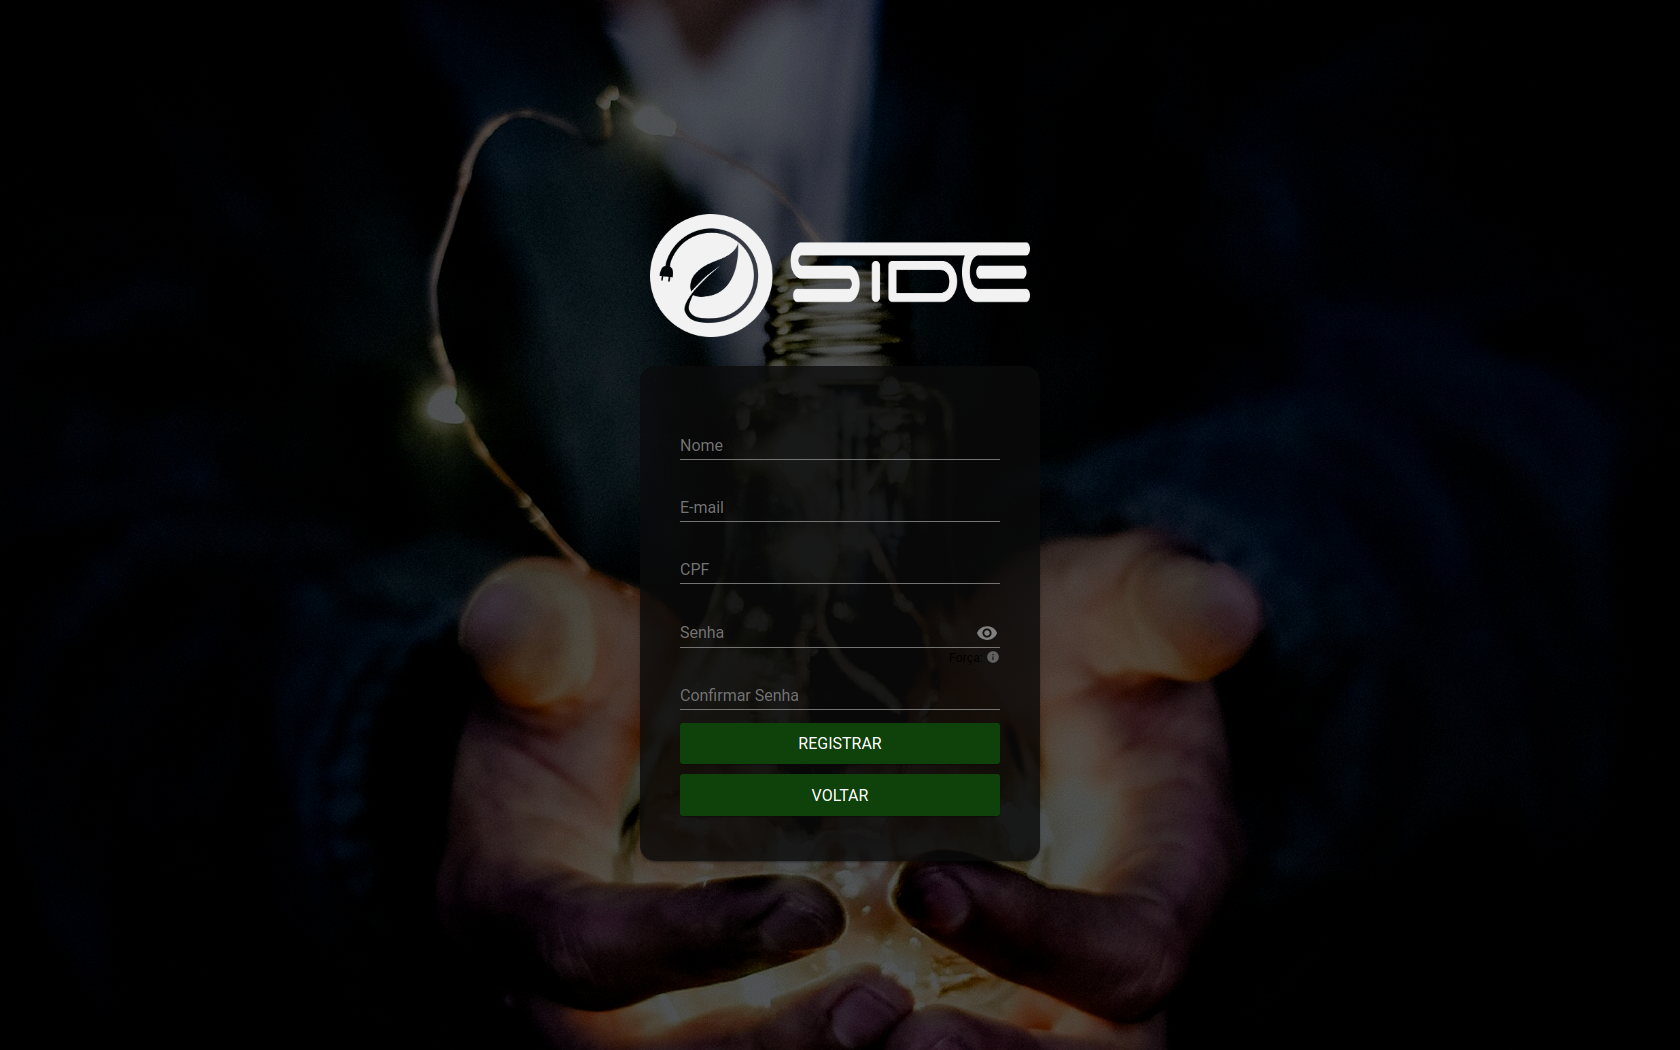
\includegraphics[width=0.65\linewidth]{imagens/side/side-cadastro.png}
    \caption*{Fonte: Próprio Autor}
    \label{fig:side-cadastro}
\end{figure}

\subsection{Tela Principal}

Após autenticado no sistema o usuário tem acesso ao uso do SIDE, onde inicialmente ele verá um mapa com todos os pontos de medição cadastrado no sistema que possuam suas coordenadas geográficas cadastradas. Esses pontos podem ser clicados, fornecendo informações mais detalhadas como consumo atual através da última leitura, denominação, data da última leitura, unidade consumidora vinculada à ele, e o tipo de medidor.

O mapa foi construído em cima de um \textit{Web Component} do Polymer fornecido pela Google para acesso a api do Google Maps. Na figura \ref{fig:side-home} temos uma imagem da \textit{home} do sistema.

\begin{figure}[H]
    \centering
    \caption{Tela Principal do SIDE}
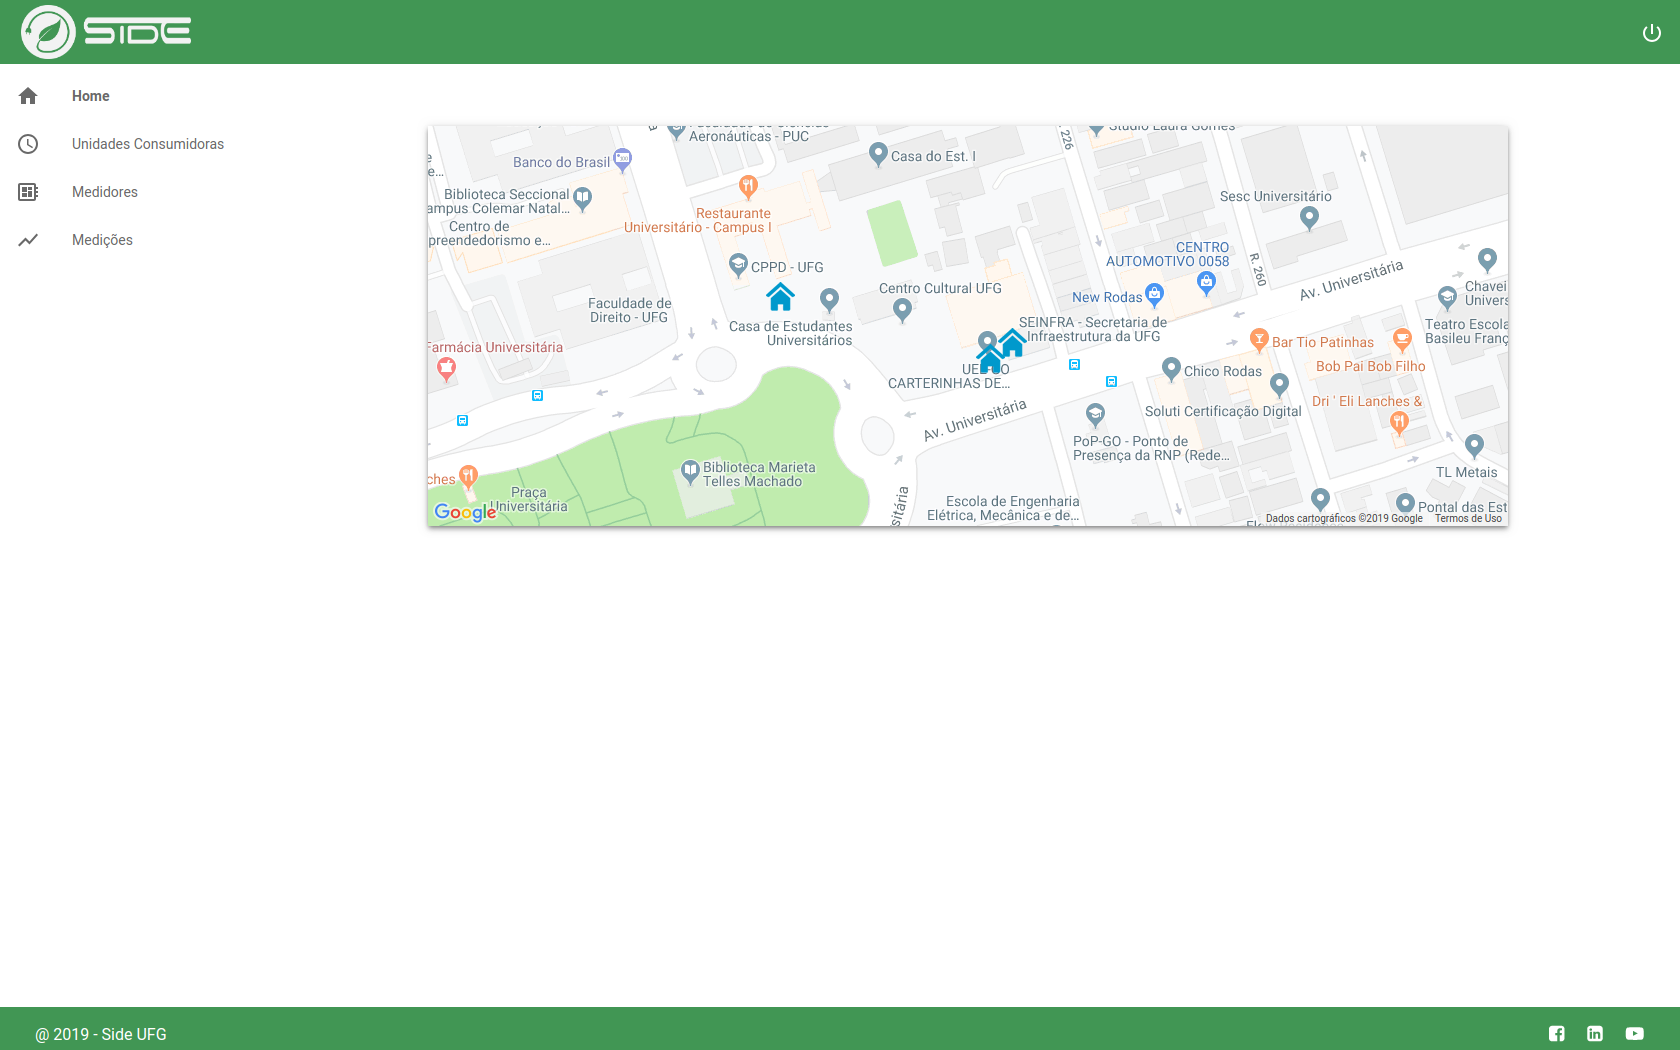
\includegraphics[width=0.65\linewidth]{imagens/side/side-home.png}
    \caption*{Fonte: Próprio Autor}
    \label{fig:side-home}
\end{figure}


\subsection{Cadastro de Unidades Consumidoras}

No menu de Unidades Consumidoras podemos visualizar os medidores da concessionária cadastrados na base, descriminados pela junção de seu nome com a número da unidade consumidora do mesmo.

Na listagem de cada unidade, pode-se ver o número do medidor e suas demandas contratadas na primeira coluna, e o endereço completo na segunda coluna. Na figura \ref{fig:side-uc-list} temos as ações disponíveis para aquele item, sendo a primeira o \textit{upload} de faturas daquela unidade consumidora, onde esta relação será validada no momento do \textit{upload}, e o segundo ícone, mostra a edição do item em si.

\begin{figure}[H]
    \centering
    \caption{Tela de Listagem das Unidades Consumidoras}
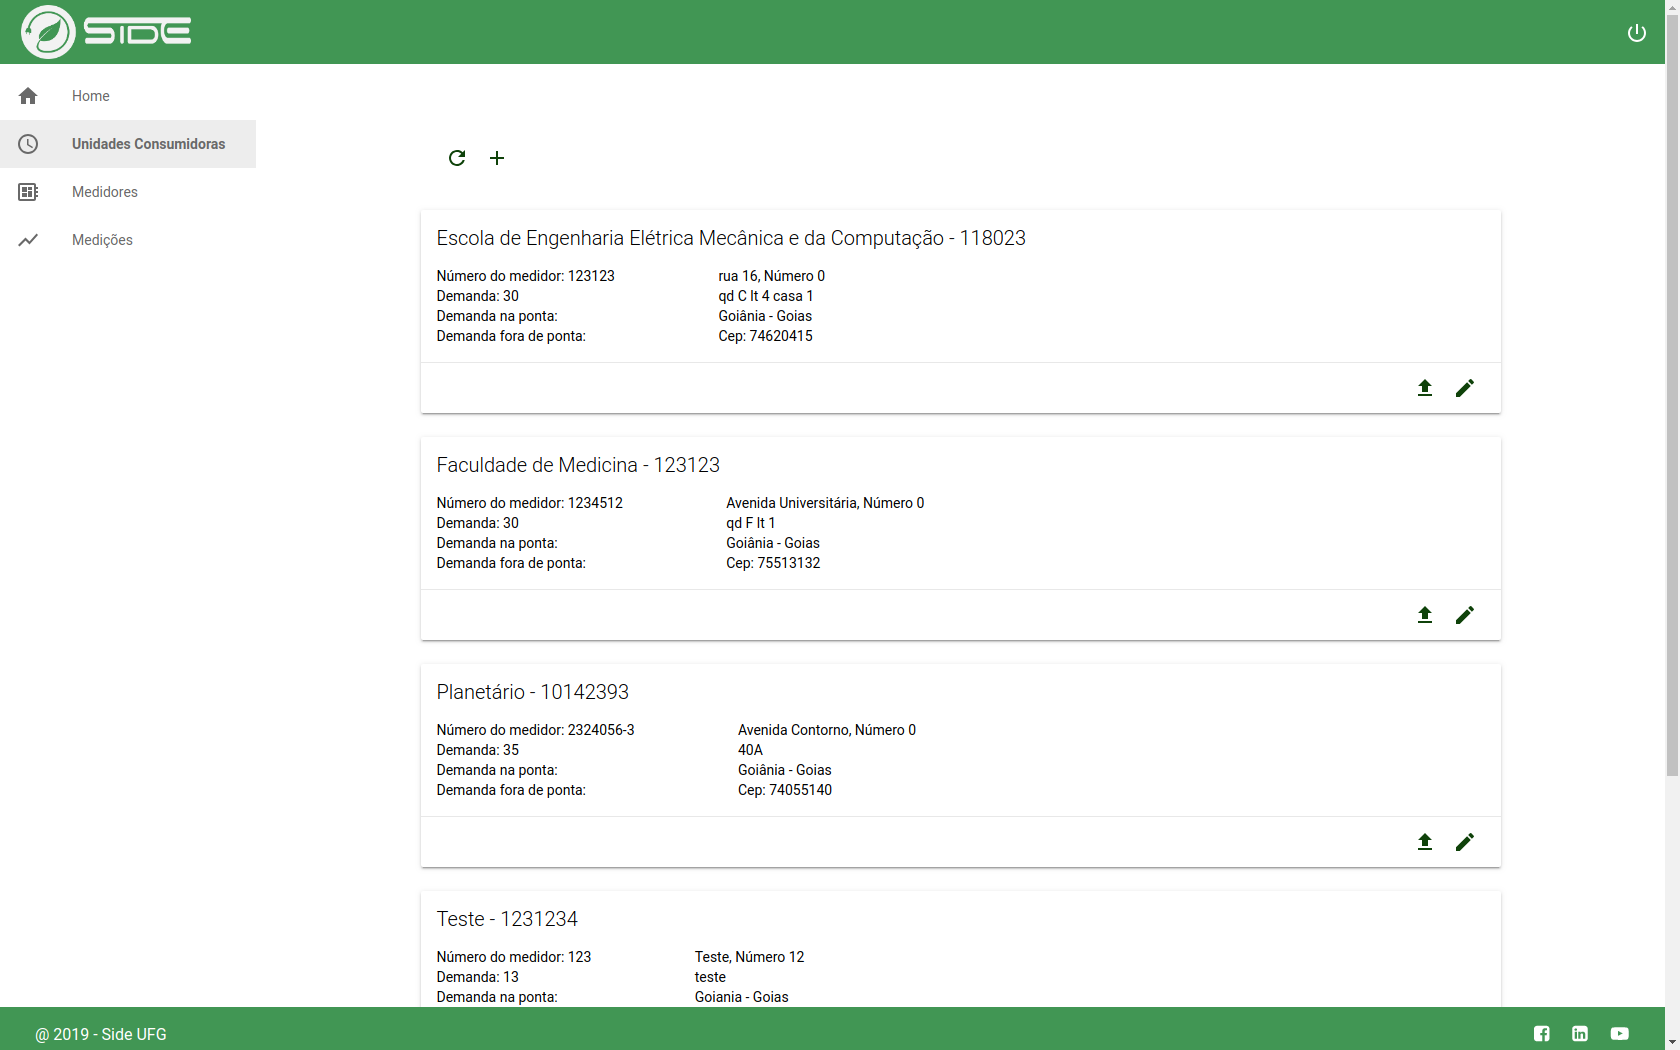
\includegraphics[width=\linewidth]{imagens/side/side-uc-list.png}
    \caption*{Fonte: Próprio Autor}
    \label{fig:side-uc-list}
\end{figure}

Ao criar uma Unidade Consumidora, através do ícone superior da tela ou editar uma através do ícone de edição do item, teremos acesso a tela de edição, onde deverão ser preenchidos os dados e após o preenchimento poderão ser salvos. Além disso é possível na tela de edição de uma unidade consumidora, apagar aquela unidade, onde a nível de banco serão desassociados todos os medidores CCK vinculados àquela unidade. 

\newpage

Na figura \ref{fig:side-uc-edit} temos uma imagem da tela de edição de unidade consumidora:

\begin{figure}[H]
    \centering
    \caption{Tela de Edição das Unidades Consumidoras}
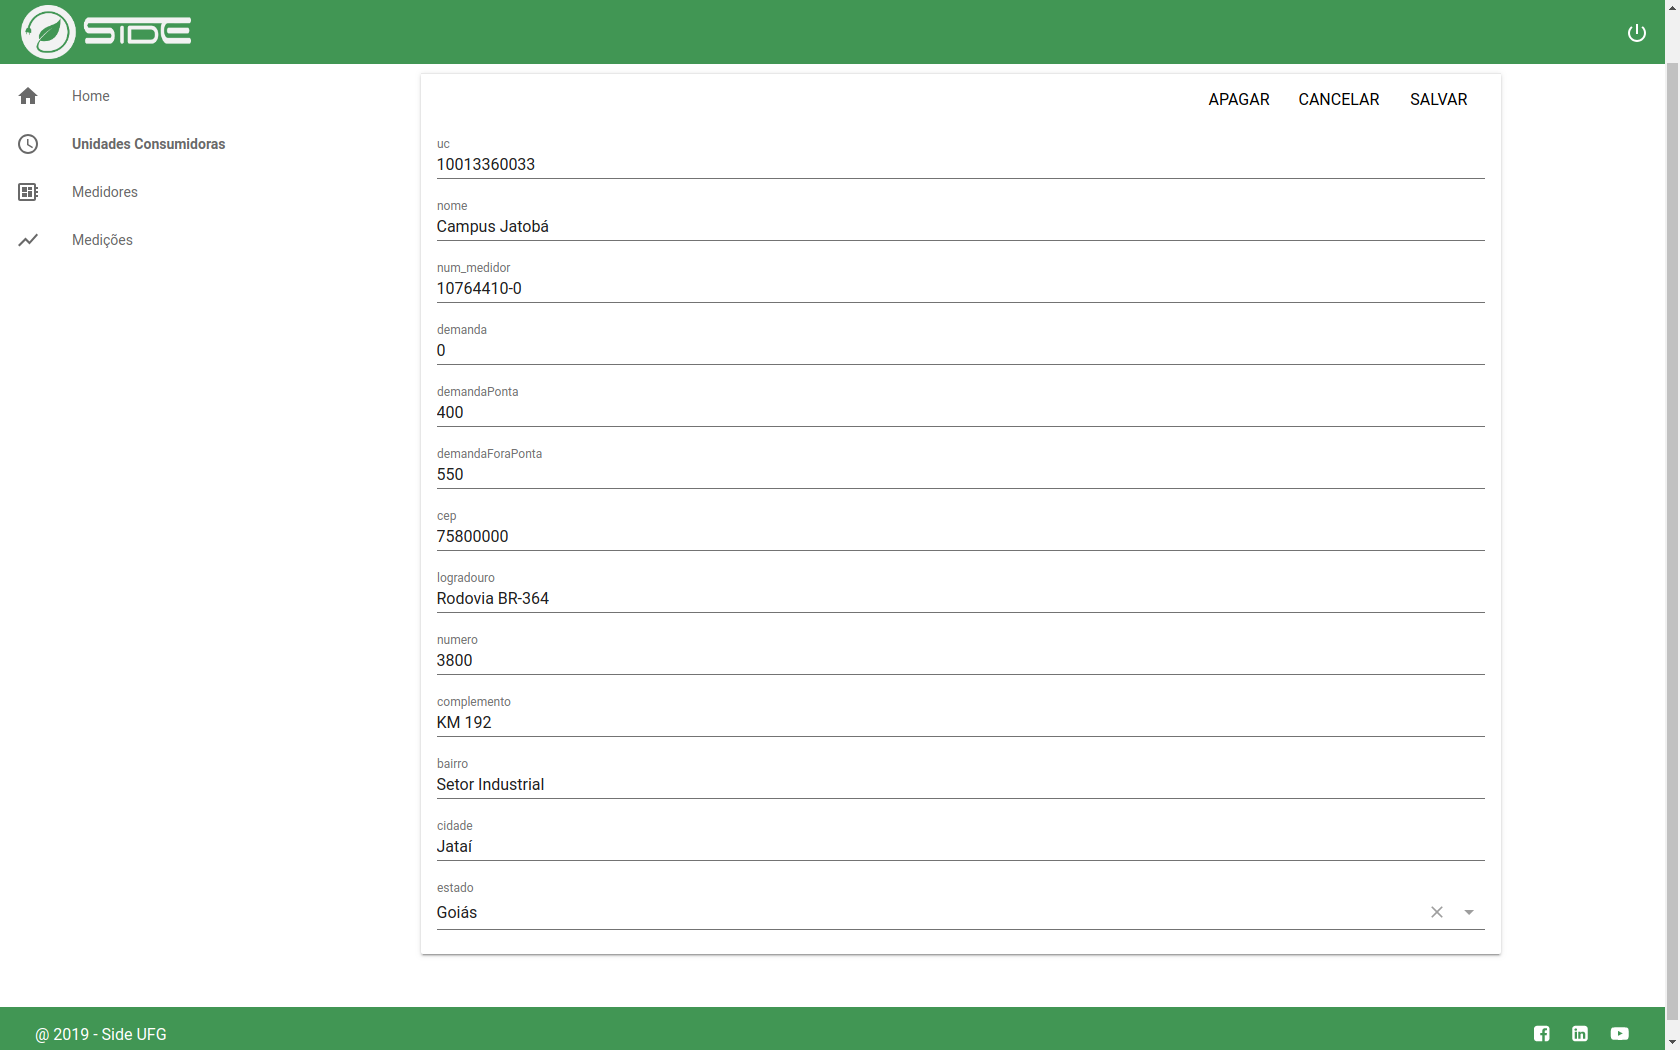
\includegraphics[width=\linewidth]{imagens/side/side-uc-edit.png}
    \caption*{Fonte: Próprio Autor}
    \label{fig:side-uc-edit}
\end{figure}

\subsection{Cadastro de Medidores}

No menu de Medidores podemos visualizar os medidores da Universidade cadastrados na base através do \textit{Side Synchronizer}, descriminados pela denominação do mesmo.

Na listagem de cada medidor, pode-se ver a unidade consumidora associada à ele, o tipo de Medidor, suas coordenadas geográficas, bem como suas datas de início e fim de leitura. Abaixo temos disponível a ação de edição para aquele item. Para a tela de medidores não é permitido cadastras ou remover itens, pois o mesmo só pode ser feito pelo dispositivo mestre da rede \textit{Modbus}.

Na figura \ref{fig:side-medidor-list} temos uma imagem da tela de listagem de medidores do sistema.

\begin{figure}[H]
    \centering
    \caption{Tela de Listagem dos Medidores CCK}
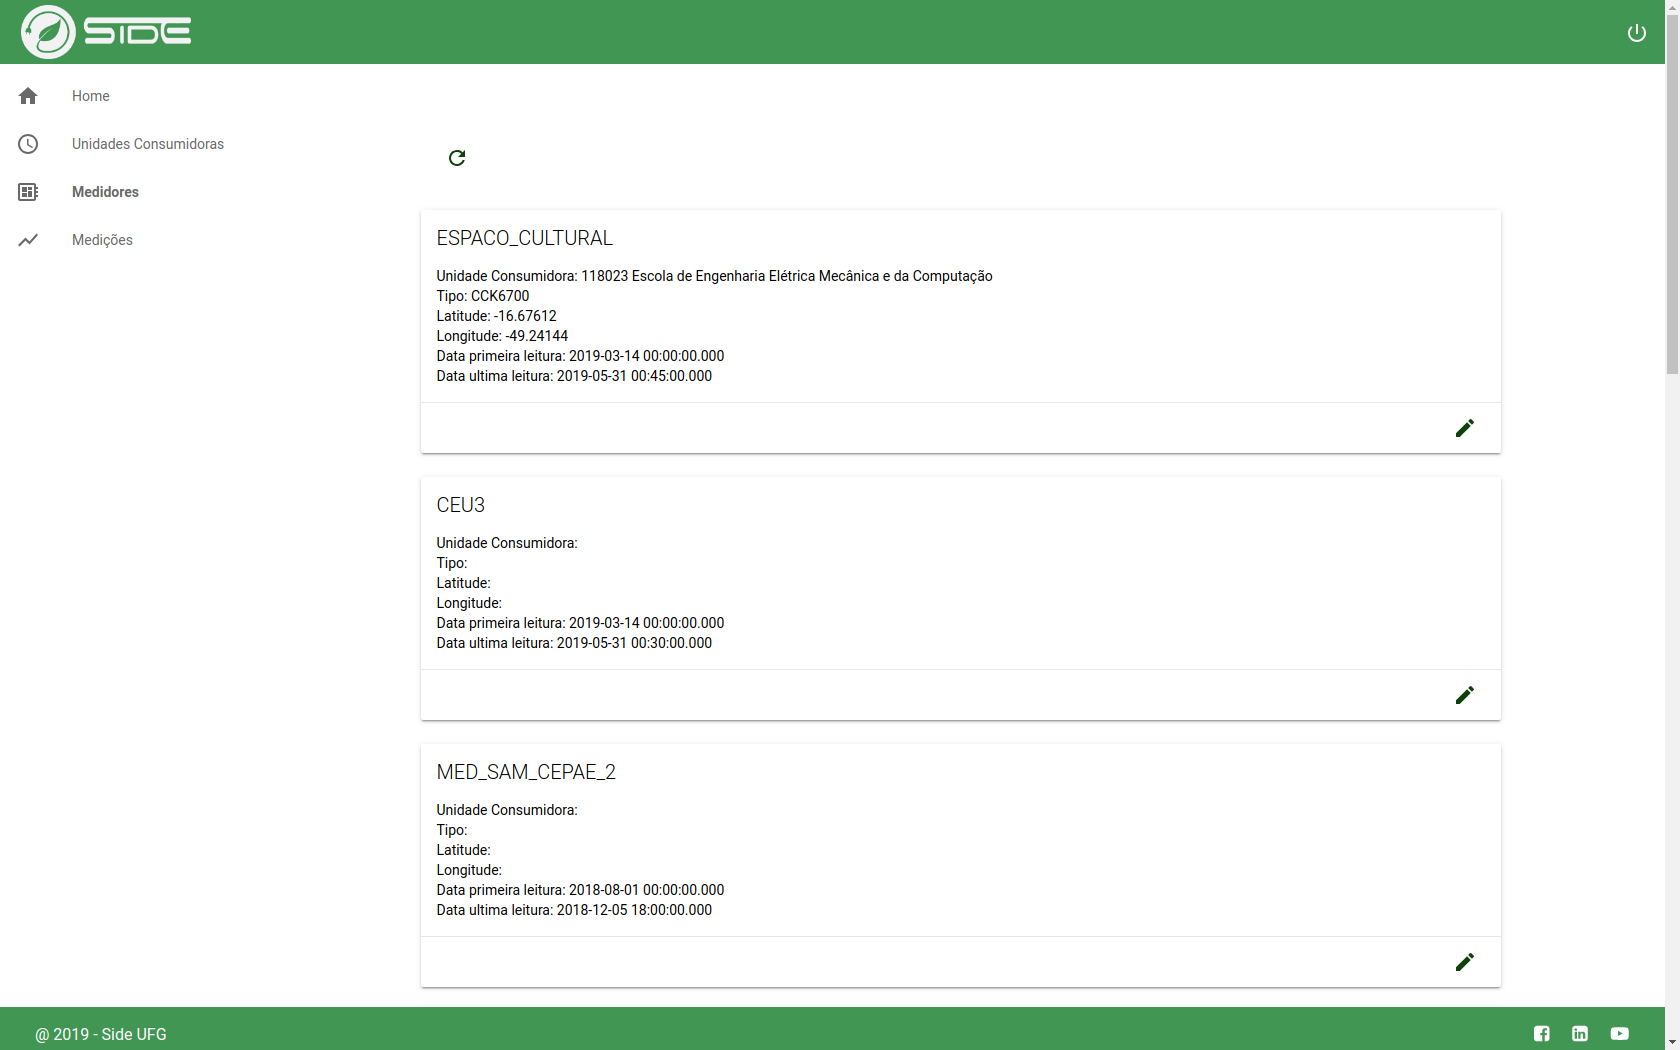
\includegraphics[width=0.75\linewidth]{imagens/side/side-medidor-list.png}
    \caption*{Fonte: Próprio Autor}
    \label{fig:side-medidor-list}
\end{figure}

Ao editar um medidor através do ícone de edição do item, teremos acesso a tela de edição, onde deverão ser preenchidos os dados e após o preenchimento poderão ser salvos. A denominação pode ser alterada pois não interfere na comunicação do \textit{Side Synchronizer} com o mestre da rede \textit{Modbus}, pois a mesma é feita utilizando o id do medidor. Por outro lado não é possível apagar aquele medidor ou criar um novo, essa ação deve ser feita pelo Gerenciador da CCK. 

Na figura \ref{fig:side-medidor-edit} temos uma imagem da tela de edição de medidor:

\begin{figure}[H]
    \centering
    \caption{Tela de Edição dos Medidores}
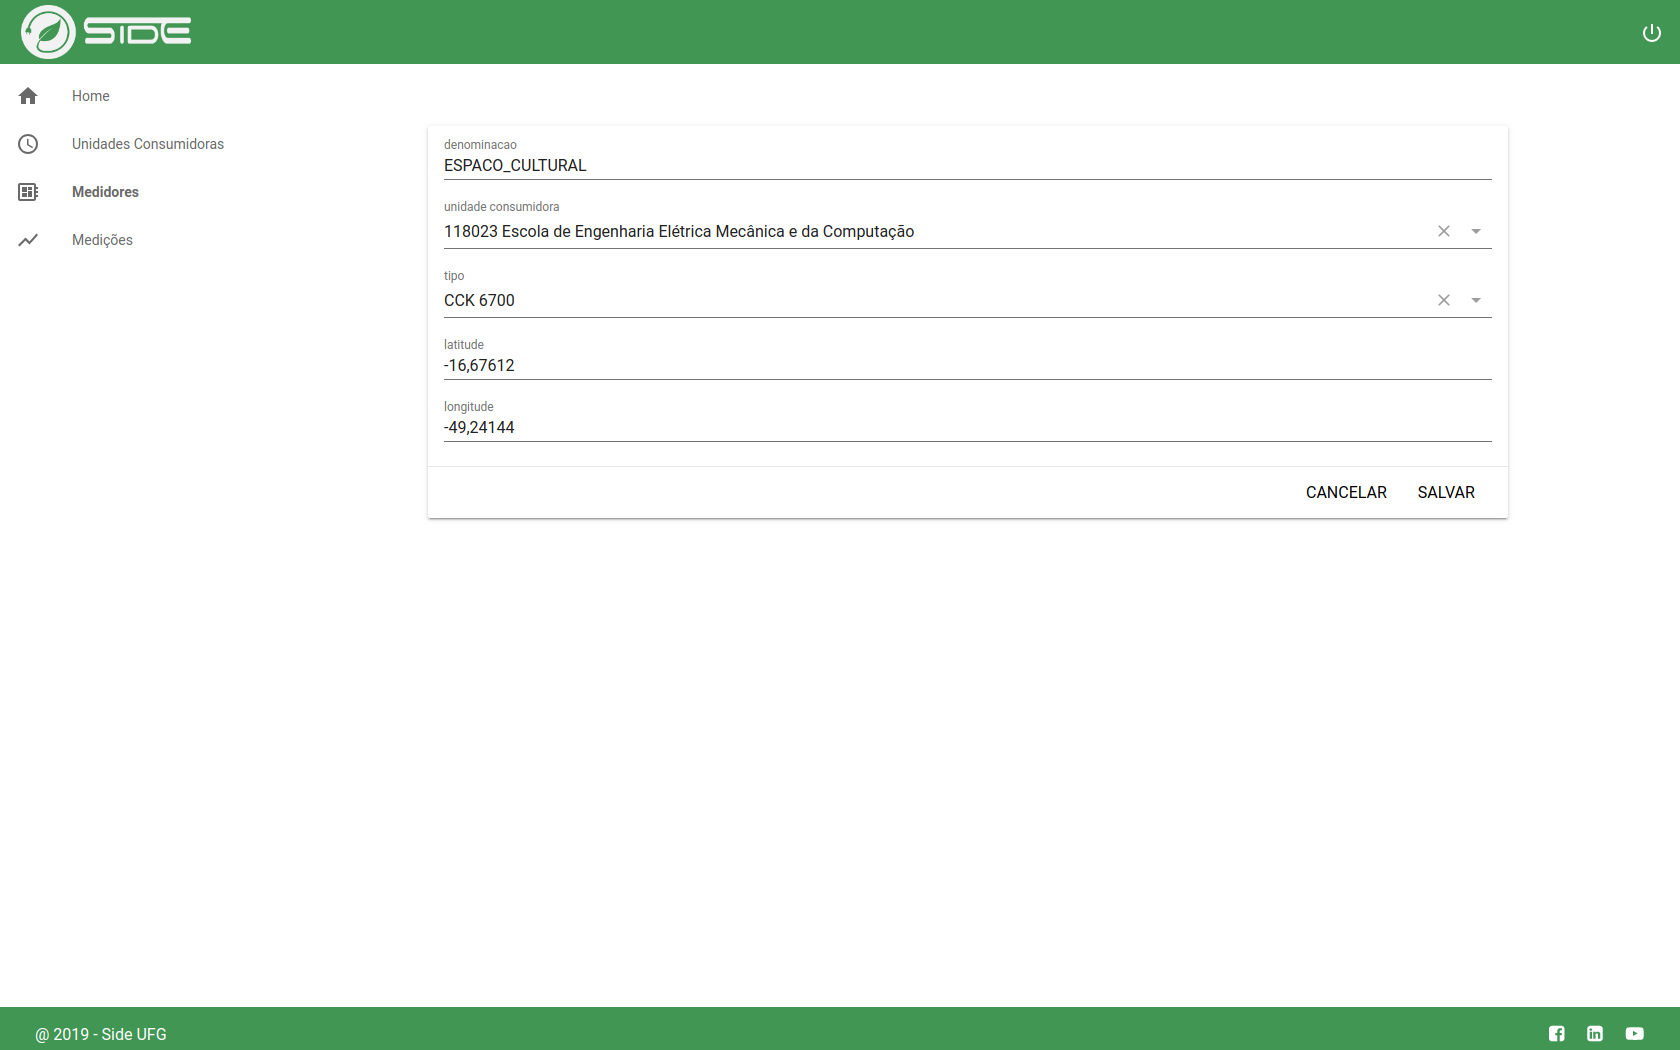
\includegraphics[width=0.75\linewidth]{imagens/side/side-medidor-edit.png}
    \caption*{Fonte: Próprio Autor}
    \label{fig:side-medidor-edit}
\end{figure}


\subsection{Visualização de Medições}

No menu de Medições podemos visualizar o gráfico das medições de um medidor da Universidade cadastrados na base através do \textit{Side Synchronizer}. Além disso as medições podem ser filtradas por data inicial e final.

Ao preencher o filtro da tela selecionando um medidor e suas datas o sistema irá buscar na tabela de medições os resultados limitados pelos parâmetros de busca. Após isso será gerado um gráfico com a curva de potência ativa e reativa distribuídos pelo tempo em um intervalo de 15 minutos.

O gráfico é interativo e permite que o usuário expanda ou comprima os eixos para detalhar melhor as leituras, além disso ao posicionar o ponteiro do mouse sobre um ponto as informações detalhadas daquele ponto serão exibidas.

Na figura \ref{fig:side-medicoes} temos uma imagem da tela de medições com o gráfico gerado através da seleção de um medidor e um intervalo de data.

\begin{figure}[H]
    \centering
    \caption{Tela de Gráfico de Medições}
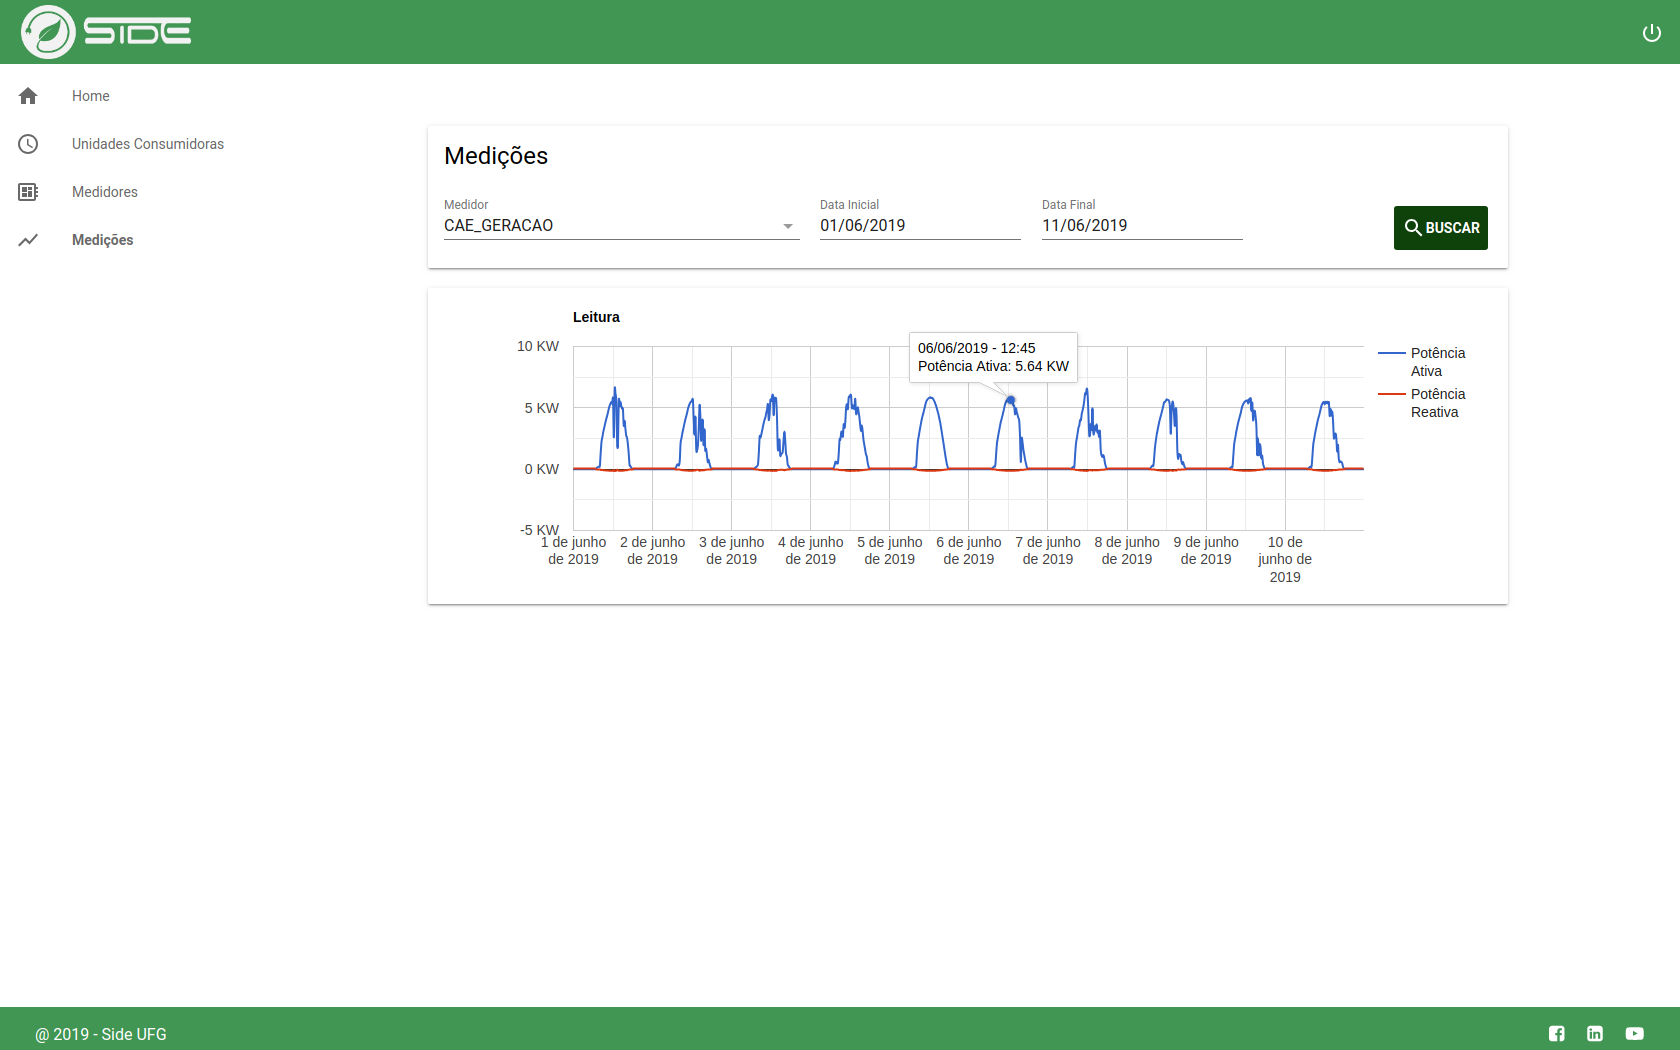
\includegraphics[width=\linewidth]{imagens/side/side-medicoes.png}
    \caption*{Fonte: Próprio Autor}
    \label{fig:side-medicoes}
\end{figure}